\documentclass[12pt]{article}

\usepackage{mathptmx}

\usepackage[colorlinks=true,urlcolor=blue]{hyperref}
\urlstyle{same}


\usepackage{graphicx}
\graphicspath{{./figures/}}

\usepackage[outdir=./figures/]{epstopdf}

\usepackage{float}

\usepackage[font=footnotesize]{caption}

\usepackage{wrapfig}

%\usepackage[a4paper]{geometry}

\usepackage{microtype}

\usepackage{booktabs}



\author{Gabriel Siqueira Kakizaki}
\date{\today}
\title{\textbf{Relationship Between Venue Categories and Income in Districts of
the City of São Paulo, Brazil}}

\begin{document}
\maketitle



\section{Introduction}

\subsection{Background}

São Paulo, according to the Globalization and World Cities (GaWC) Research Network, is an alpha global city, along with Los Angeles and Amsterdam. São Paulo ranks among the wealthiest and the most populous cities, known for its cultural, social, and ethnic diversity. Often holding international events, it is sought-after because of its business opportunities.


\subsection{Problem}

Opening a new business in such a place can be challenging for several reasons. Choosing a store location is a complex process that should consider multiple factors; income is one of them. This project aimed to discover the relation between the type of venue and the income of people living in São Paulo's districts.


\subsection{Stakeholder interest}

The main audience of this project are entrepreneurs choosing where to open a business in São Paulo. The results are potentially useful for real estate agents, investors, or people just wanting to reallocate.


\section{Data}

\subsection{Data sources}

Income and geographic data came from IBGE (Brazilian Institute of Geography and
Statistics), and can be accessed
\href{https://www.ibge.gov.br/en/home-eng.html}{here}. Specifically, the
income data comes from the 2010 Census (details provided here:
\href{https://www.ibge.gov.br/en/statistics/social/income-expenditure-and-consumption/18391-2010-population-census.html?=&t=o-que-e}{here}),
and geographic data comes from
\href{https://www.ibge.gov.br/geociencias/organizacao-do-territorio/malhas-territoriais/26565-malhas-de-setores-censitarios-divisoes-intramunicipais.html?=&t=o-que-e}{here}
(portuguese) in form of shapefiles, the geographic information system (GIS)
software.  Venue data was gathered using the
\href{https://developer.foursquare.com/places}{Foursquare Places API} with a
free account created for this project.

\subsection{Data description}

\subsubsection{Geographic data}

Shapefiles have information about the district boundaries, along with
its name, code, and id. Data covered the whole state of São Paulo, not just
the city. A sample of the data is shown in \autoref{fig:geopandas}.

\begin{figure}[h]
        \centering
        \includegraphics[width=0.8\textwidth]{geopandas.png}
        \caption{Geopandas dataframe\label{fig:geopandas}}
\end{figure}

\subsubsection{Census data}

The census table contained various attributes and the statistics columns were
labeled with ``VXXX'', where XXX was a three-digit number. The relationship
between the labels and their meaning can be found in the 2010 census documentation.

As we were interested only on the income for this project, only the column ``V009'' was used:
``Value of the average nominal monthly income of people aged 10 and over (with and without income)'' (Freely translated from Portuguese). This column had no missing values.

Originally, each row is associated with a unit called ``census sector''
(Portuguese: setor censitário), which is generally a lot smaller than the actual
district, composed only of one or a few city blocks.

The data format can be seen in \autoref{fig:census_table}.

\begin{figure}[h]
        \centering
        \includegraphics[width=\linewidth]{census_table.png}
        \caption{Structure of the IBGE census data.\label{fig:census_table}}
\end{figure}

\subsubsection{Venues}

# It's your decision to write this section in the first voice. Passive voice is okay even though harder to read.

Foursquare API was used to collect the name, category, latitude and longitude
values for a total of 8036 venues in a 2 km radius around the centroid of each
of the 96 districts. The results returned from the API in JSON format were
merged into a dataframe containing the district name, and coordinates as shown
in \autoref{fig:venues_table}.

\begin{figure}[h]
        \centering
        \includegraphics[width=\linewidth]{venues_table.png}
        \caption{Pandas dataframe containing the venue information.\label{fig:venues_table}}
\end{figure}



\section{Methods}

Data processing, analysis and modeling were performed using Python. This project is available as a Jupyter notebook at my github page
(\href{https://github.com/kakig}{github.com/kakig}).
\verb!Coursera_Capstone!.

\vfill

\subsection{Exploratory data analysis (EDA)}


# Make this map bigger. It's beautiful and you shoud use it in your favor.

\begin{wrapfigure}{L}{0.5\textwidth}
        \centering
        \includegraphics[width=\linewidth]{map_centroids.png}
        \caption{Map of São Paulo showing districts with markers on its
        centroids.\label{fig:map_centroids}}
\end{wrapfigure}

As shapefiles came with information for the whole state, only data about the
city was selected. Then, centroids were calculated for each district using its
geometric information, for use with the Foursquare API.\spacefactor\sfcode`.{}


Conversion between different coordinate reference systems (CRS) was needed
for this calculation and for plotting maps, which also required generating a
GeoJSON object. To validate that the area and placement of the districts and the
centroids were correct, a map was created for visualization, as
shown in \autoref{fig:map_centroids}.


Census data also required processing. To get the average income per district, data were grouped by district name and the mean value was taken.
The mean income for the districts was R\$1576.82, and the minimum and maximum
as R\$396.48 and R\$5402.81, respectively. There were a few outliers, but they had not influenced the analysis. The distribution of the
values can be seen in \autoref{fig:plot_income}.

# Please, remove gridlines. They suck. Make the backgroud white too. Use colors wisely.


\begin{figure}[htb]
        \centering
        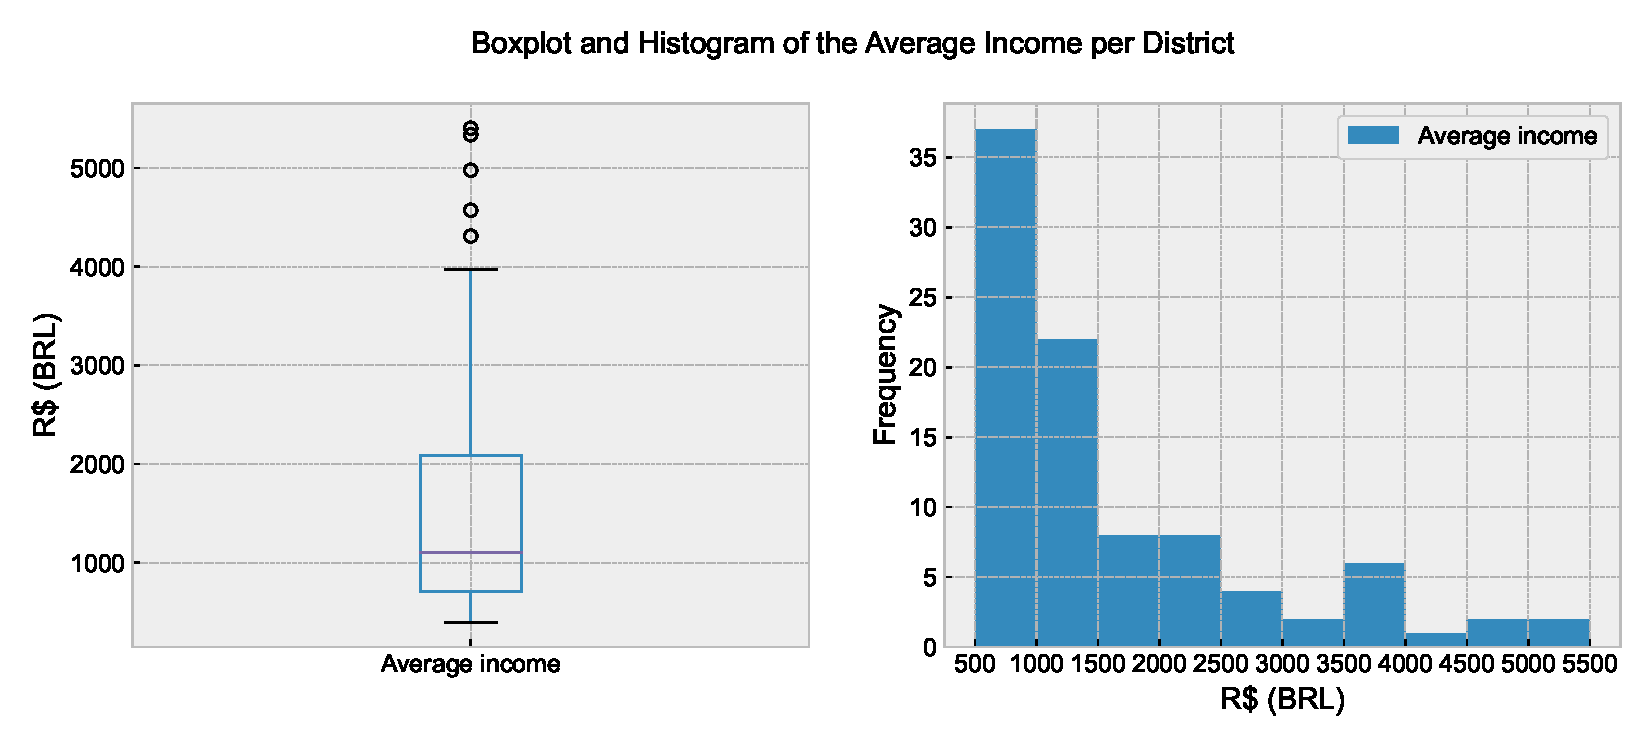
\includegraphics[width=\linewidth]{plot_income.eps}
        \caption{Boxplot (left) and histogram (right) of income. Values in
        Brazilian Real.\label{fig:plot_income}}
\end{figure}

# Don't hide this incredible map. Make it bigger.

\begin{wrapfigure}{R}{0.5\textwidth}
        \centering
        \includegraphics[width=\linewidth]{map_income.png}
        \caption{Average income per district of São Paulo. Red means higher
        income.\label{fig:map_income}}
\end{wrapfigure}

In \autoref{fig:map_income}, we can observe that
 income is more concentrated towards the city center. If the income has no impact on the type of venues, then we would expect that venus are scattered across the map uniformly.
 

# Begin your paragraphs with a topic setence. Cut the clutter.

# Bad. Switching focus to working with venue information, due to the difference in

# Good. Venue data had also to be processed. First, I did... Second, I did... You may keep the passive tense if you like; harder to read though.
 
 
# Rewrite this para...

Switching focus to working with venue information, due to the difference in
number of venues between districts, first, one-hot encoding was used to
transform the table, keeping only the category value for each venue. There were
363 unique venue categories that became the columns for the table. Data in this
format were used to visualize the most common venues in the whole city. Then, the
values were grouped by district with and the mean was taken, so we ended up with
the frequency of venue categories in percentage for each district. This may
allow for a better and more fair comparison during modeling.


\subsection{Modeling}

Machine learning models were built using the
\href{https://scikit-learn.org/stable/index.html}{scikit-learn} library. Both
unsupervised (K-Means) and supervised (Lasso, Random Forest) learning approaches
were used.

\begin{wrapfigure}{l}{0.5\linewidth} \centering
        \includegraphics[width=\linewidth]{plot_elbow.eps}
        \caption{Elbow method for choosing the number of clusters in
        K-Means\label{fig:plot_elbow}}
\end{wrapfigure}

K-Means algorithm was used to segment \emph{n} data points (districts) into
\emph{K} segments, or clusters, with similar characteristics (venue frequency).
Note that income data \textbf{was not} used to train this algorithm. As it
cannot automatically determine the number of clusters in the data, the elbow
method was used for choosing the optimal \emph{K}, which was three in this
case.


The target of prediction for regression was the mean income for each district.
Due to our sample size, models were evaluated using \emph{k-fold}
cross-validation (\(k=5\)) to estimate the coefficient of determination (R²),
the mean absolute error (MAE) and the root mean squared error (RMSE).

Lasso was used instead of ordinary least squares regression due to the large
number of features (363 venue categories), as it tends to have fewer non-zero
coefficients, thus being simpler.

Random forest was also used because it doesn't have the same prior assumptions as Lasso (i.e., attributes and features are linear related). In this particular case, a decision tree model might fit the data better while providing insight into each feature's importance.


\section{Results}

\subsection{Clustering}

# Add a topic sentence first. Example: Three clusters were found using the elbow method...


K-Means segmented the districts mainly into 2 clusters, and the third cluster
contained only one district, the most southern one which contains an
environmental preservation area, and because of that it was excluded from
further analysis.

\begin{figure}[h]
        \centering
        \includegraphics[width=\linewidth]{map_cluster_labels.png}
        \caption{Choropleth map of income per district. Dark purple circles
        indicate the district is part of the first cluster, and yellow circles,
        the second.\label{fig:map_cluster_labels}}
\end{figure}

\newpage

The first cluster had 55 districts with a mean income of R\$924.24 and the
second had 40 districts, and a mean income of R\$2503.62, more than double than
the first one. The first cluster also had mostly bakeries and pizza places as the
most common venues, while the second had a more diverse selection of venues. As seen in \autoref{fig:map_cluster_labels}, districts
from the second cluster are usually located more to the center.

%\autoref{tab:clusters} shows the number of districts and the income for the
%first two clusters. The first cluster had 55 districts with a mean income of
%R\$924.24 and the second had 40 districts, and a mean income of R\$2503.62,
%more than double than the first one. The first cluster also had mostly bakeries
%and pizza places as most common venues, while the second had a more diverse
%selection of most common venues.

%\begin{table}[h]
%        \centering
%        \begin{tabular}[c]{ c c c }
%                \toprule
%                Cluster & Districts & Mean Income (R\$) \\
%                \midrule
%                1 & 55 & 924.24 \\
%                2 & 40 & 2503.62 \\
%                \bottomrule
%        \end{tabular}
%        \caption{Number of districts and mean income from clusters\label{tab:clusters}}
%\end{table}

\subsection{Regression}

\begin{table}[h]
        \centering
        \begin{tabular}[c]{ c c c c }
                \toprule
                Model & R² (mean, std) & MAE & RMSE \\
                \midrule
                Lasso & 0.53 (0.19) & 615 & 810 \\
                Random Forest & 0.58 (0.15) & 566 & 752 \\                \bottomrule
        \end{tabular}
        \caption{Coefficient of determination, mean absolute error and root
        mean squared error for lasso and random forest
        models.\label{tab:models}}
\end{table}

\autoref{tab:models} shows the performance of the two regression models. Random
forests performed better than Lasso in all metrics, thus it was used to explain
which venue categories are correlated with high and low income districts using
SHAP values as shown in \autoref{fig:plot_shap_rf}. We can see that higher
bakery frequency tends to lower the value of the predicted income, confirming
what was shown with clustering. In general, restaurants of different (foreign)
cuisines are related to a value increase of the outcome, indicating that
they are located in higher income areas.

It is also interesting to see that spa, vegetarian/vegan restaurant and art
museum categories impact positively the model output, reinforcing the common
belief that these places are frequented by people with higher economic status.

\begin{figure}[h]
        \centering
        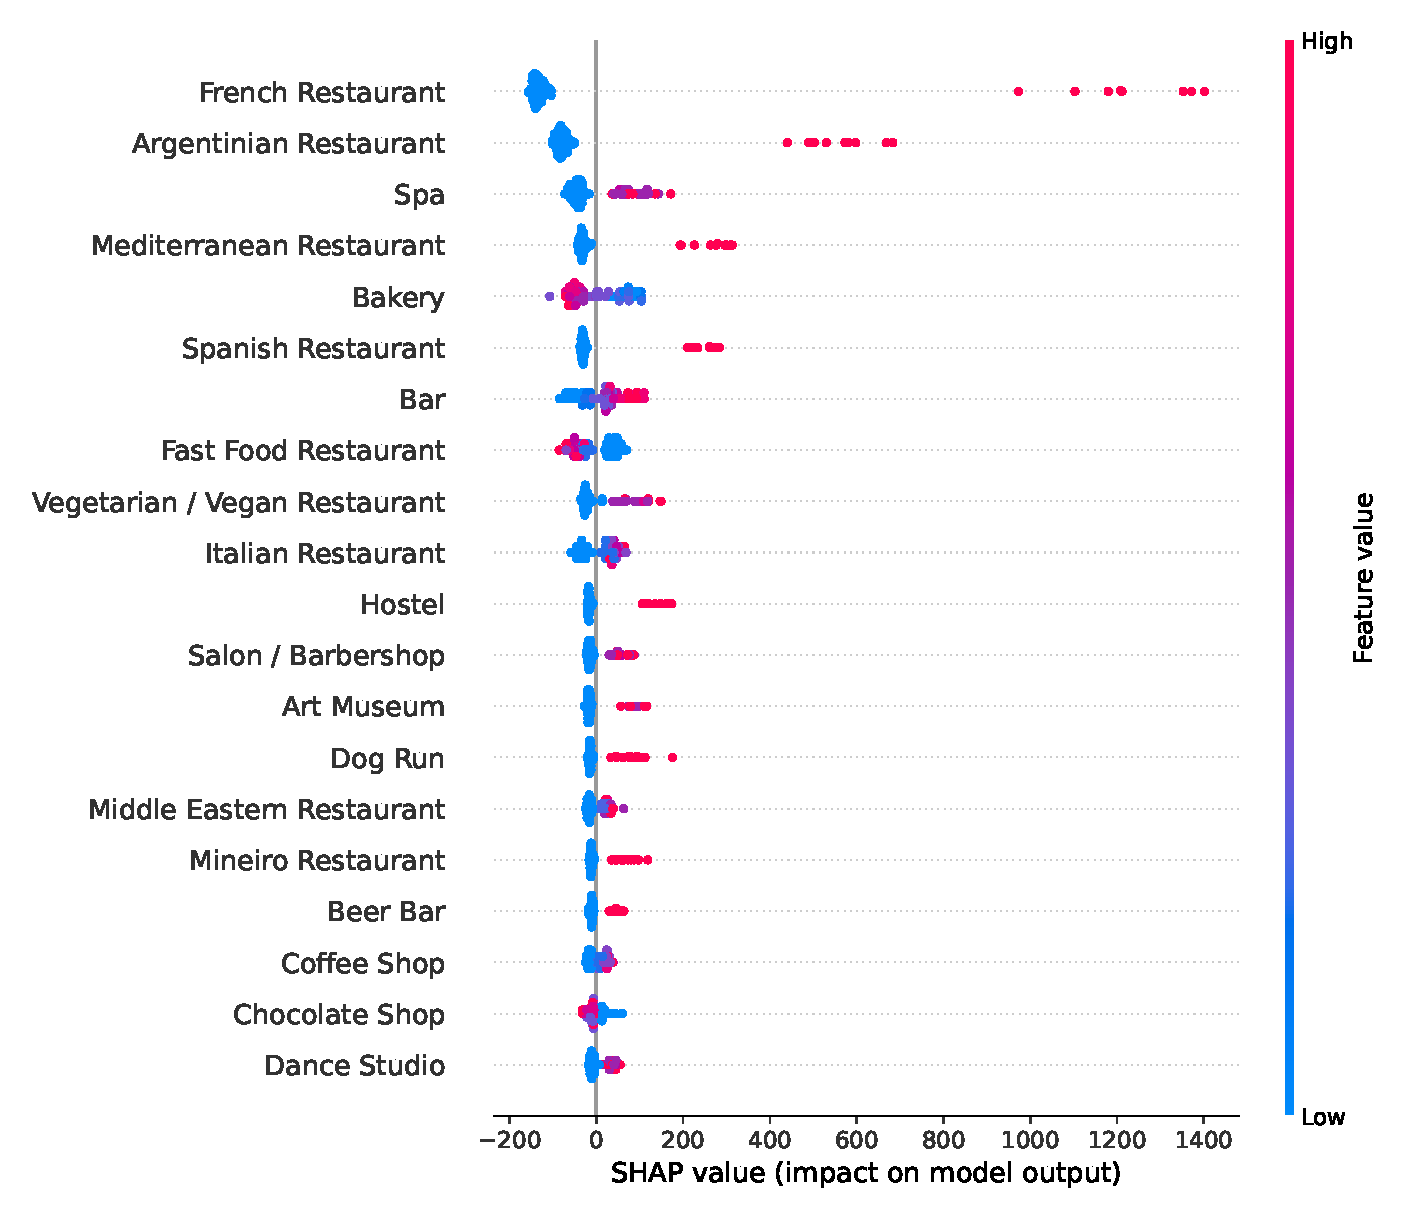
\includegraphics[width=\linewidth]{plot_rf_shap.eps}
        \caption{SHAP values for the top 20 features sorted by average impact
        on model output.\label{fig:plot_shap_rf}}
\end{figure}



\section{Discussion}

\subsection{Recommendations}

Further projects should focus on the relationship between venue types and other kinds of
data, such as crime rates and rent prices. This might
lead to other insights about venue localization and answer the project goal. Also, using a smaller unit of analysis than a district could be
useful for pinpointing more exact locations suited for opening a new business.

While working with geographical data, caution should be used to verify that the
information about all places is correct. I faced issues with districts, and
previously with neighborhoods that had the exact same name in this and other
cities. Yet, the names can contain abbreviations and sometimes do not match
where they should.

\subsection{Limitations}

The census data was gathered in 2010, and venue data is from 2020. This may
impact the models accuracy and the explanations of which venue types are
correlated with higher or lower income areas.

Venue data was gathered in a 2 km radius from the district centroids, because
the Foursquare API is limited to a circular search around latitude and
longitude coordinates. This 2 km radius was good for most of the districts, although far from ideal. Venue data for smaller districts agglomerated
in the center may have included venues in other adjacent districts, and
districts at the edge of the city might have venues from other cities, due to
conurbation. While I could have restricted venues to be inside of the district,
this would result in less data for the machine learning algorithms, and in
practice, these kinds of political divisions aren't really obstacles for people
going to the venues.

\section{Conclusion}

In this study, I analyzed the relationship between the venue categories and the
income for districts of São Paulo. I identified that a few venue
categories are correlated to income, especially restaurants from foreign
cuisine. It is also worth noting that bakeries and fast-food restaurants appear
more frequently in lower income areas. This information can be useful to help
entrepreneurs deciding the location of a new business.

\end{document}
